\chapter{Entity-level Sentiment Analysis}
\label{chap:entity-level-sentiment-analysis}
This chapter focuses on entity-level sentiment analysis and includes concise experiments. Using our named entity recognition algorithm described in Chapter \ref{chap:comapny-to-symbol-linking}, we identify organisations along with their corresponding ticker symbols. Instead of presenting naive approaches that involve holistically parsing sentences where entity mentions occur and subsequently analysing only sentiment-determining keywords associated with those entities, we describe and partially modify an algorithm based on the FinABSA model, which we have chosen as the foundation for our sentiment analysis.

We also discuss the challenges associated with finding a suitable dataset to validate our algorithm. Finally, we present the results of our experiment using the FinEntity dataset, which contains paragraphs from newspaper articles, entity annotations, and corresponding sentiments. For the sentiment analysis, we achieved a success rate of $92\%$. However, it is essential to note that this high accuracy was obtained after significantly reducing the original dataset to ensure precise measurement. 

Additionally, we explore the correlation between entity-level sentiment and adjusted close prices of stocks, demonstrating promising relationships that underline the potential of sentiment analysis in financial markets. A detailed analysis of these experiments is available in a dedicated Python notebooks\footnote{Located in the directory /ipynbs/entity-level-sentiment-analysis/.} that provides comprehensive insights into our methodology and findings.

\section{Introduction}
\label{sec:elsa-introduction}
At the current stage, leveraging our named entity recognition algorithm discussed in Chapter \ref{chap:comapny-to-symbol-linking}, we have identified entities, specifically organizations and their corresponding tickers, which we refer to as companies. The algorithm selectively filters these companies to include only those listed on specific exchanges, namely NASDAQ, NYSE, and AMEX. This section focuses on sentiment analysis at the entity level within these exchanges.

We will omit naive approaches involving sentiment analysis, where sentences mentioning an entity are analyzed holistically through the whole sentence. Such approaches may yield partial insights assuming a single entity per sentence, attributing uniform sentiment to all mentioned entities. However, these methods overlook whether keywords related to sentiment within sentences are associated with the entity.

Another comparable approach is entity-level sentiment analysis, where sentences are considered based on keywords determining sentiment in coexistence with the mentioned entity. This method offers efficiency and addresses challenges posed by multiple entities within a single sentence, establishing a direct link between keywords and entities. Nevertheless, complications may arise in interpreting keywords with ambiguous sentiments linked to other words so that their meaning can vary and deepen, relying on the other words, such as in the simple example of ``\textit{like}'' and ``\textit{not like}''.

\section{FinABSA model}
\label{sec:elsa-finabsa-model}
Instead of considering naive approaches, we will focus on slight modifications to meet the needs of our sentiment analysis algorithm implementation based on the FinABSA model\footnote{\href{https://www.github.com/guijinSON/FinABxwSA}{https://www.github.com/guijinSON/FinABSA}}. This model was trained specifically for the financial domain using the SEntFiN 1.0 dataset \parencite{sentfin}. Even though the model is considered aspect-based, where aspects refer to targets as ``\textit{[TGT]}'', its practical application extends to entity-level sentiment analysis by defining these targets through any tagging mechanism. The model excels at handling multiple entities across sentences and enables numerical sentiment analysis. To derive an overall entity's sentiment score and distribution, it categorises sentiments into positive, neutral, and negative classes based on the highest value ranging from $0$ to $1$.

The model is available in two versions, namely FinABSA\footnote{\href{https://www.huggingface.co/amphora/FinABSA}{https://www.huggingface.co/amphora/FinABSA}}, which shows lower performance with longer sentences, and FinABSA-Longer\footnote{\href{https://www.huggingface.co/amphora/FinABSA-Longer}{https://www.huggingface.co/amphora/FinABSA-Longer}}, which should be able to handle more extended sentences. Due to the length of articles we are dealing with, we have chosen the extended version. However, both versions are constrained by a token limit of $512$. Therefore, in our algorithm adaptation, we process input articles in chunks, each containing a maximum of $512$ tokens. It is crucial to avoid splitting sentences based on token count into two parts to prevent loss of context and ensure accurate analysis. If a last sentence exceeds the token limit within a chunk, it is taken into the subsequent chunk. These chunks are processed in parallel, and their outcomes are consolidated as a collected result. The final sentiment determination for each entity is derived from the highest averaged class scores.

Regarding entity tagging, we leverage our already mentioned entity recognition algorithm. This algorithm guarantees entities representing companies with the ticker. Each identified entity is then mapped to a target ``\textit{[TGT]}'', enabling the model to recognise companies and perform sentiment analysis accordingly.

\section{Experiment: FinEntity Dataset}
\label{sec:elsa-experiment-finentity-dataset}
Obtaining a suitable dataset to validate the correctness of our algorithm presents significant challenges, such as the necessity of at least text excerpts from news articles, including companies as entities and their associated sentiments. Publicly available datasets possessing entire articles are almost impossible to obtain. There are enough datasets containing entity information concerning tweets or article headlines focusing on single-entity contexts, proving non-optional for our experimental needs because both tweets and headlines have a different structure than articles.

Creating our dataset would be excessively time-consuming or monetarily expensive if relying on human annotators. Nevertheless, the work \parencite{tang-etal-2023-finentity} describes the development of a FinEntity dataset, available on Hugging Face\footnote{\href{https://www.huggingface.co/datasets/yixuantt/FinEntity}{https://www.huggingface.co/datasets/yixuantt/FinEntity}} built on the financial domain with the contribution of financial experts. This dataset contains $979$ paragraphs sourced from newspaper articles, each annotated with entities and their corresponding sentiments. Notably, each paragraph may encompass multiple entities with their associated sentiments. Despite the dataset containing only excerpts rather than entire articles, it remains the most suitable option for our experiment.

The entities within the FinEntity dataset consist of companies without explicit information on their details about exchange listings. Consequently, our named entity recognition algorithm is restricted to NASDAQ, NYSE, and AMEX entities. Thus, we must filter out from dataset entities not traded on these exchanges. In addition, some annotations do not have information about the associated ticker. Thus, we must remove these entities to determine whether they are traded on the exchanges we consider in our named entity recognition algorithm. Table \ref{table:elsa-entities-finentity-summary} gives the specific entity counts, which do not consider unique entities - taking into account entity occurrences and duplicate entities as well. After filtering, $540$ entities remain available for our experiment, distributed across $282$ paragraphs out of $979$ (see Table \ref{table:elsa-paragraphs-finentity-summary}).

\begin{table}[ht]
    \centering
    \caption{Entities summary in FinEntity dataset. (Note: Including duplicates.)}
    \label{table:elsa-entities-finentity-summary}
    \begin{tabular}{l c}
        \hline
        \multicolumn{2}{c}{\textbf{Entities}} \\
        \cline{1-2}
        Description & Count \\
        \hline
        Total & 2,131 \\
        Without ticker & 1,359 \\
        With ticker & 772 \\
        \textbf{On specified exchanges} & \textbf{540} \\
        \hline
    \end{tabular}
\end{table}

\begin{table}[ht]
    \centering
    \caption{Paragraphs before and after cleaning summary in FinEntity dataset.}
    \label{table:elsa-paragraphs-finentity-summary}
    \begin{tabular}{l c}
        \hline
        \multicolumn{2}{c}{\textbf{Paragraphs}} \\
        \cline{1-2}
        Description & Count \\
        \hline
        Before cleaning & 979 \\
        \textbf{After cleaning} & \textbf{282} \\
        \hline
    \end{tabular}
\end{table}

Our named entity recognition approach recognised $460$ entities, each of which does not necessarily equal any of the $540$ already annotated entities in the dataset. Our entities include, for example, those that did not contain a ticker and were removed from the annotations as a result. 

Upon closer examination, it becomes evident that inconsistencies in annotation, such as Tesla sometimes being tagged with a ticker and sometimes without, contribute to the variation in the number of entities retrieved. This inconsistency also obscures unrecognised entities due to the limited context provided by the shorter paragraphs.
Some entities were not identified by our named entity recognition algorithm because they did not progress to the stage of querying Wikidata. For instance, Johnson \& Johnson\footnote{\href{https://www.wikidata.org/wiki/Q333718}{https://www.wikidata.org/wiki/Q333718}}, despite having stock exchange NYSE information listed on Wikidata, was not recognised as an organisation by the spaCy tagger. The Entity Linker may also need more information about the entity, resulting in an undetermined QID. Our methodology currently employs only three query variants over the SPARQL data. If the Entity Linker identifies an entity as Johnson \& Johnson (United Kingdom)\footnote{\href{https://www.wikidata.org/wiki/Q30338424}{https://www.wikidata.org/wiki/Q30338424}}, we could enhance accuracy by incorporating a query that considers the ``\textit{parent organisation}'' property. This would ensure that the primary entity, Johnson \& Johnson, which contains the relevant stock exchange information, is correctly recognised.

However, this section primarily focuses on entity-level sentiment analysis to evaluate sentiment. After extracting entities, our sentiment analysis algorithm, rooted in the FinABSA-Longer model, processes these entities to determine their sentiment. Before presenting the results of the experiment, we describe three perspectives that we focus on to evaluate the results for each paragraph:

\begin{description}
    \item [Matched]: The number of entities with the same ticker and entity's text that have the same sentiment in the dataset and our annotations.
    \item [Unmatched]: The number of entities with the same ticker and entity's text that have different sentiments in the dataset and our annotations.
    \item [Unfound]: The number of entities that are in the dataset but not in our annotations.
\end{description}

Table \ref{table:elsa-proportion-matched-unmatched-unfound} and Figure \ref{fig:elsa-proportion-matched-unmatched-unfound} show that the number of matched entities is $287$, representing $53.1\%$. There are also $25$ unmatched entities whose sentiment did not match the dataset, accounting for $4.6\%$, and $228$ entities not found in our annotations, making up $42.2\%$. The success percentages may seem low if we only consider these unmatched entities. Thus, focusing only on sentiment evaluation, the results are entirely sufficient, with a success rate of $287$ out of $312$, or $92.0\%$ (see Figure \ref{fig:elsa-proportion-matched-unmatched}).

\begin{table}[ht]
    \centering
    \caption{Results of entity-level sentiment analysis. The proportion of Matched, Unmatched, and Unfound entities.}
    \label{table:elsa-proportion-matched-unmatched-unfound}
    \begin{tabular}{l c}
        \hline
        \multicolumn{2}{c}{\textbf{Entities}} \\
        \cline{1-2}
        Description & Count \\
        \hline
        Matched & 287 \\
        Unmatched & 25 \\
        Unfound & 228 \\
        \hline
    \end{tabular}
\end{table}

\begin{figure}[htpb]
    \centering
    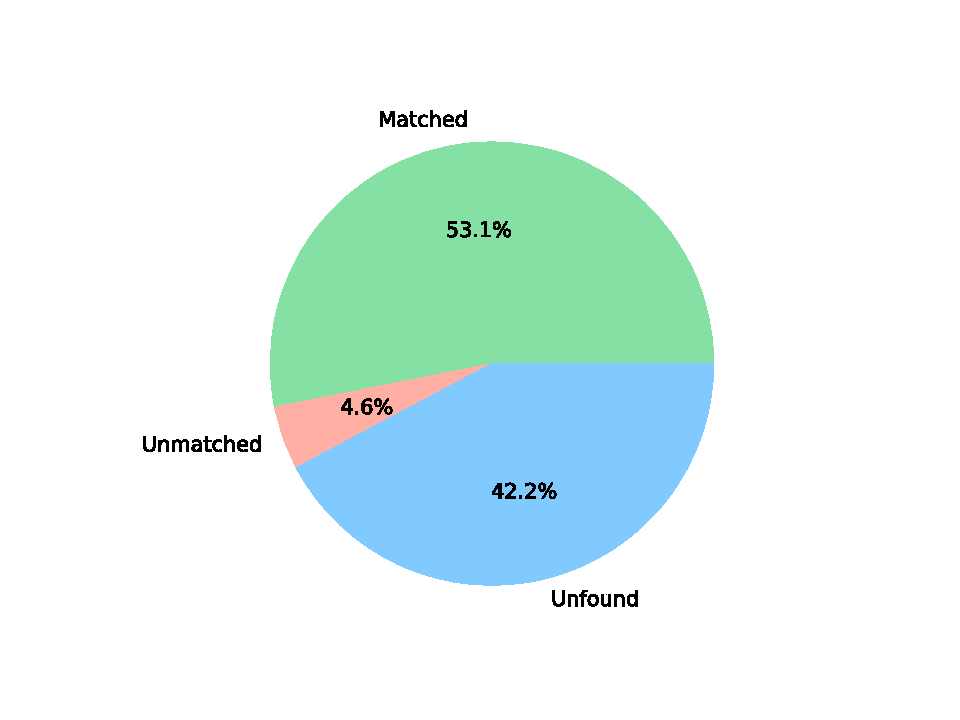
\includegraphics[width=0.9\textwidth]{img/elsa/proportion_matched_unmatched_unfound-a.pdf}
    \caption{The pie chart shows the result proportion of Matched, Unmatched, and Unfound entities.}
    \label{fig:elsa-proportion-matched-unmatched-unfound}
\end{figure}

\begin{figure}[htb]
    \centering
    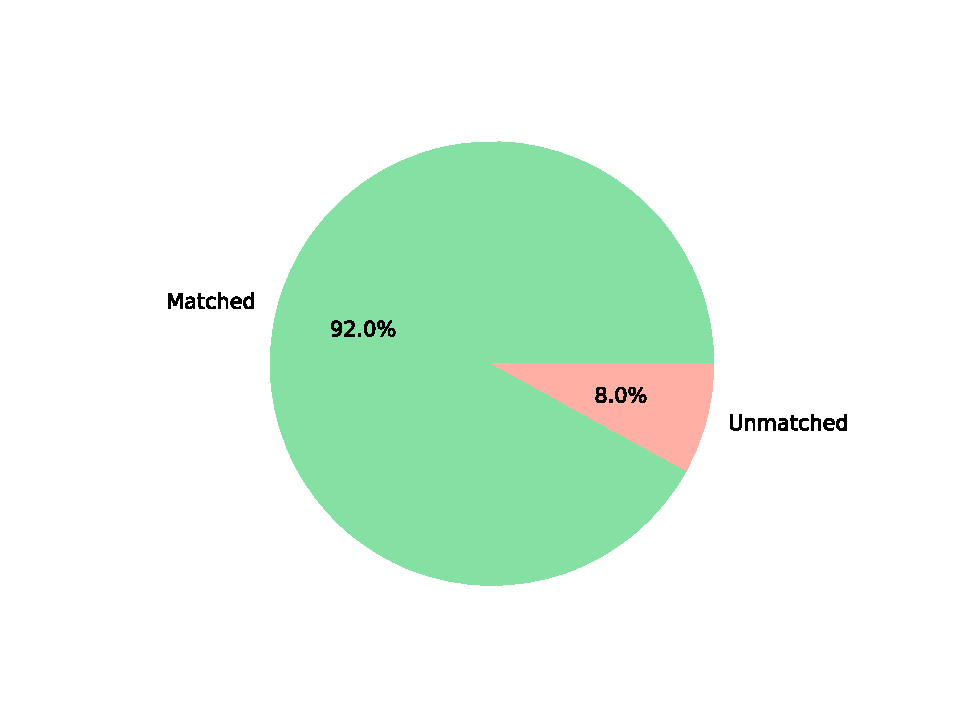
\includegraphics[width=0.9\textwidth]{img/elsa/proportion_matched_unmatched-a.pdf}
    \caption{The pie chart shows the result proportion of Matched and Unmatched entities.}
    \label{fig:elsa-proportion-matched-unmatched}
\end{figure}

\section{Experiment: Sentiment and Adjusted Close Price}
\label{sec:elsa-experiment-stock-price-correlation}
Once we have built an algorithm to extract companies and their associated sentiment from the text, we can analyse how sentiment value and stock price are related. For this purpose, we utilise the Yahoo Finance Python library\footnote{\href{https://www.pypi.org/project/yfinance/}{https://www.pypi.org/project/yfinance/}} to obtain historical stock adjusted close price \parencite{adj_close_bib} of companies based on their ticker symbols. The news articles are sourced from the Guardian, providing us with enough data including whole content for analysis. We focus on articles from the business and technology sections published in the first quarter of $2024$, from January $1$ to March $31$.

The data, such as articles from the business and technology sections, are published inconsistently. Multiple articles may be published on any given day. In such cases, we will consider the average sentiment of all articles. We assign the sentiment value to the next market day if an article is published on a non-market day, such as a weekend or holiday. The data from the original distribution of articles before aggregation is shown in Figure \ref{fig:elsa-experiment-stock-nvda-preaggregated}, and after aggregation in Figure \ref{fig:elsa-experiment-stock-nvda-aggregated}. The figures illustrate the results of the sentiment analysis of the company Nvidia Corp. (NVDA) evaluated by our named entity recognition algorithm and using the modified FinABSA-Longer model. The company's sentiment is divided into positive, neutral, and negative components, totalling a value of $1$.

\begin{figure}[htbp]
    \centering
    \begin{subfigure}{0.8\textwidth}
        \centering
        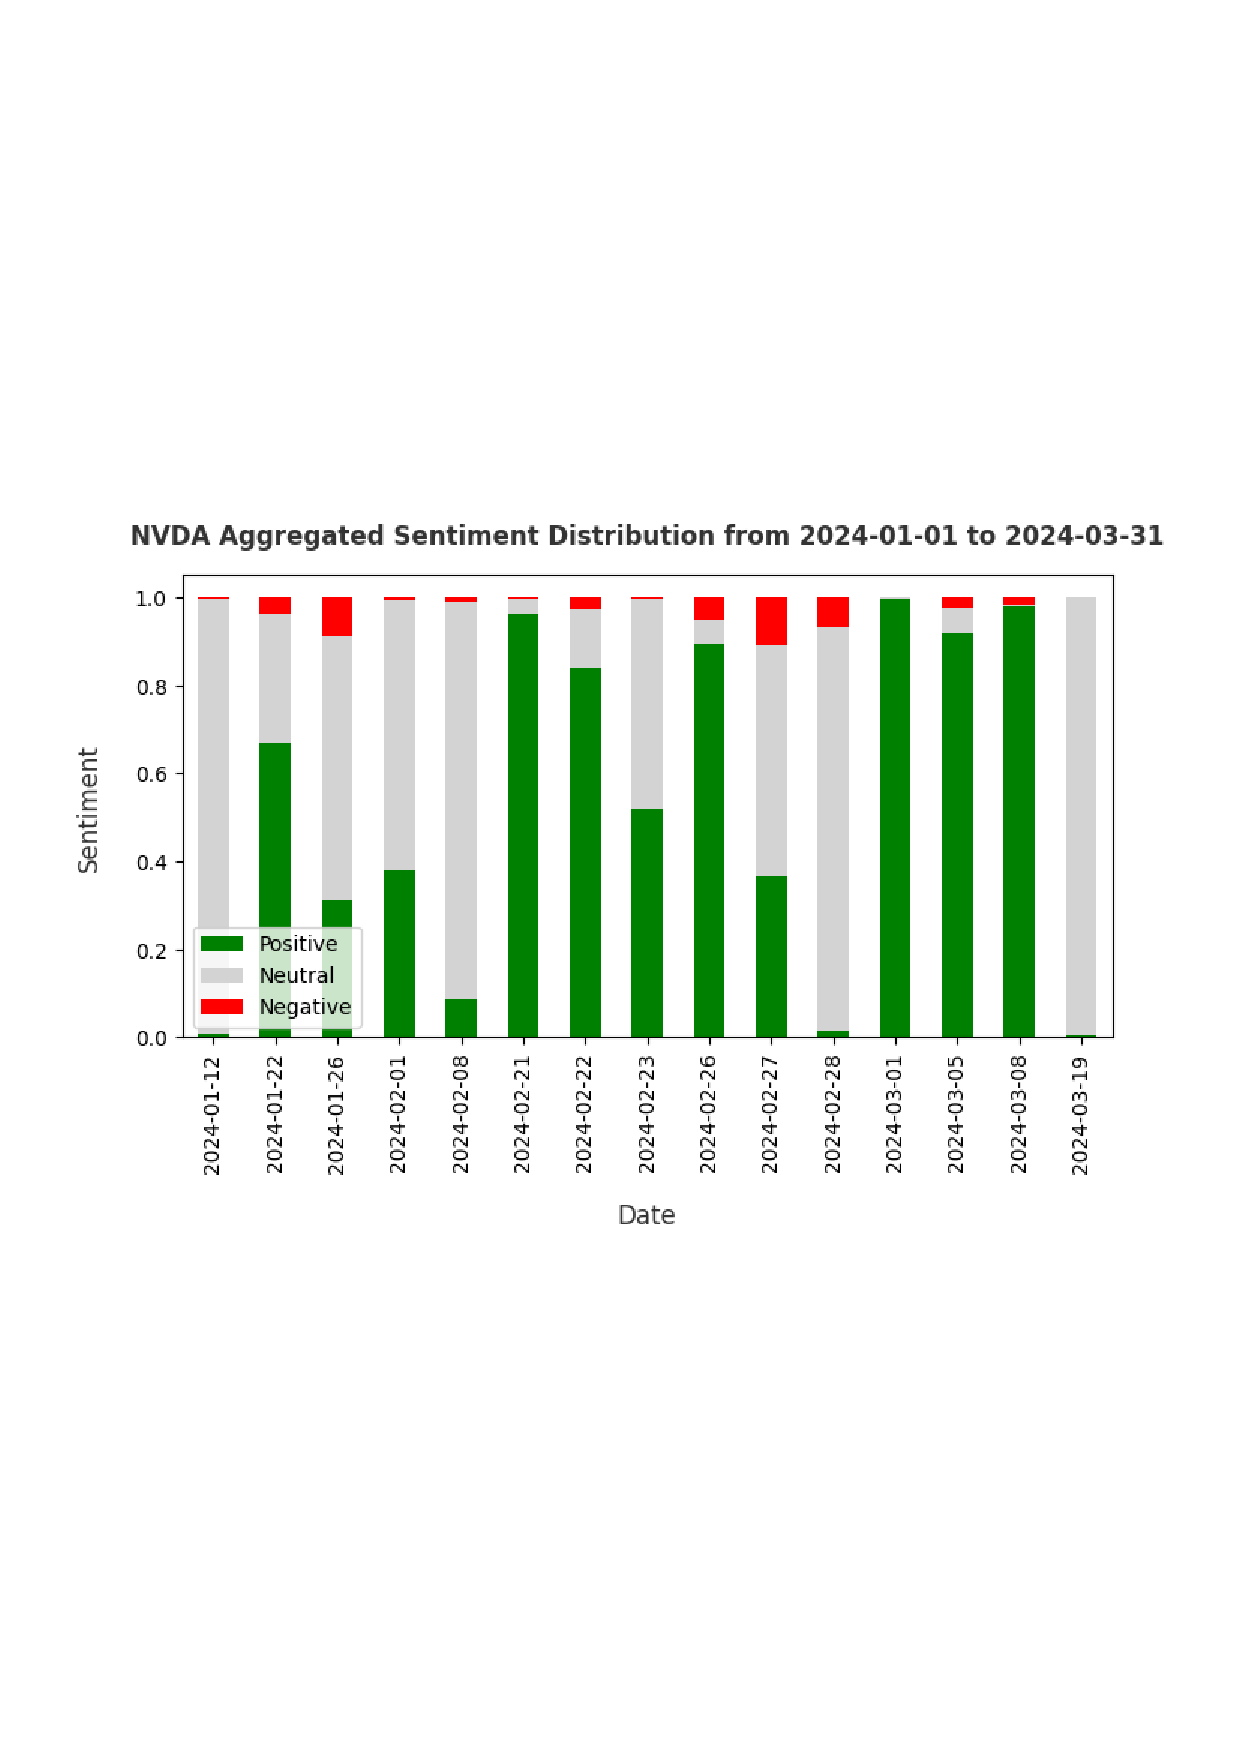
\includegraphics[width=\textwidth]{img/experiment-stock/nvda-preaggregated-a.pdf}
        \caption{Distribution of sentiment before aggregation.}
        \label{fig:elsa-experiment-stock-nvda-preaggregated}
    \end{subfigure}
    \hfill
    \begin{subfigure}{0.8\textwidth}
        \centering
        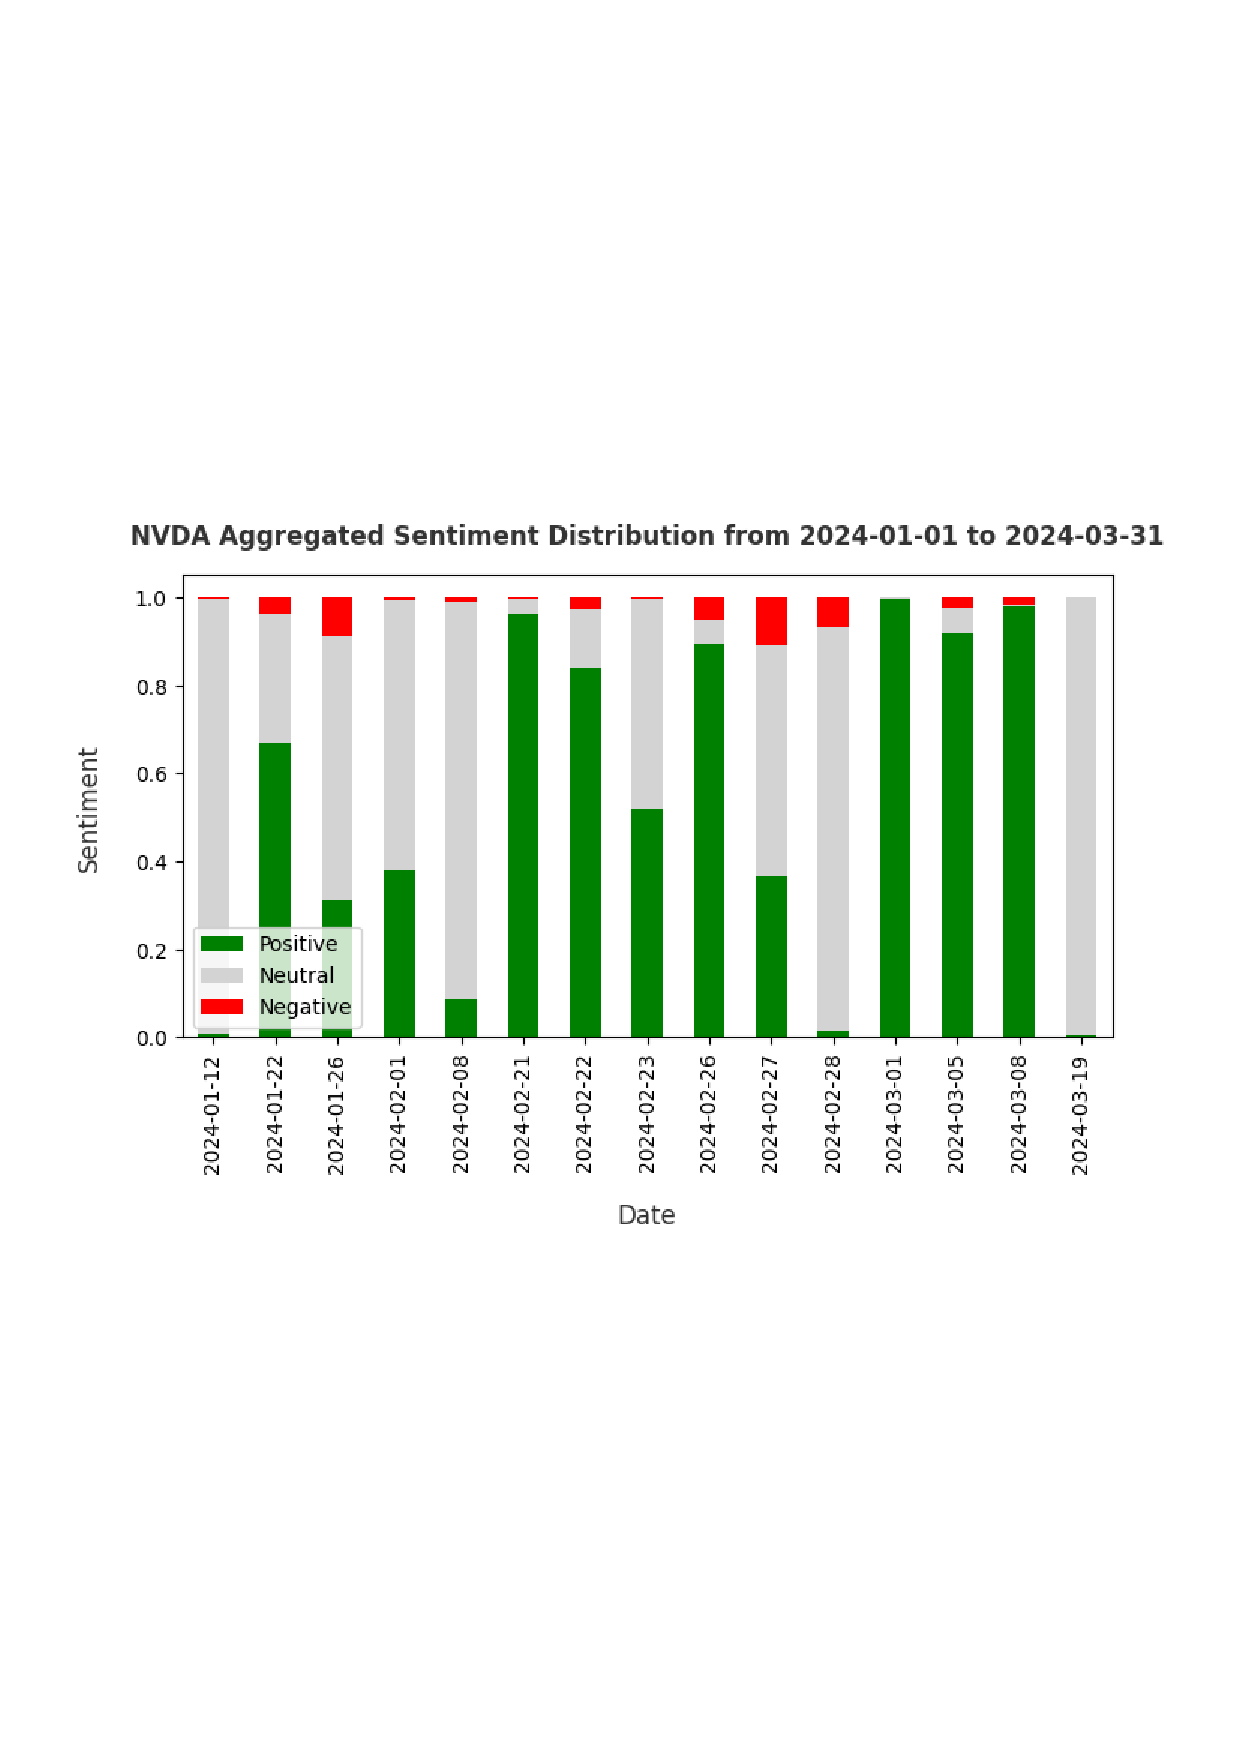
\includegraphics[width=\textwidth]{img/experiment-stock/nvda-aggregated-a.pdf}
        \caption{Distribution of sentiment after aggregation.}
        \label{fig:elsa-experiment-stock-nvda-aggregated}
    \end{subfigure}
    \caption{The sentiment analysis of Nvidia Corp. (NVDA) in the first quarter of 2024.}
    \label{fig:elsa-experiment-stock-nvda-comparison}
\end{figure}

It is worth reminding the basis behind our choice of entity-level sentiment analysis. Rather than assessing the overall sentiment of an entire article, we focus specifically on the sentiment related to Nvidia. This distinction is crucial because the overall sentiment of an article may not accurately reflect the sentiment toward individual companies mentioned within it. Providing sentiment analysis on the entity level gives investors more precise and actionable insights.
 
For instance, if we were to evaluate the sentiment of an entire article without isolating the sentiment tied to specific companies, the resulting sentiment score could be misleading. An article might have a generally negative tone but still contain positive sentiments about Nvidia, or vice versa. Our approach ensures that the sentiment value reflects only the sentiments pertinent to a single company, making it a reliable indicator for investors.

\subsection{Hold Strategy}
\label{subsec:elsa-hold-strategy}
A positive sentiment towards a company typically suggests a potential rise in its stock price. Consequently, if the sentiment analysis indicates a predominantly positive sentiment, it would be classified as positive, a potential buy opportunity marked as a buy signal. Conversely, if the analysis reveals a predominantly negative sentiment, it would be classified as negative, suggesting a sell signal. If the sentiment is predominantly neutral, it would be classified as neutral, indicating without action.

Let us define a simple, straightforward holding strategy without using any other indicators. Buy and sell signals from previous day trigger corresponding position entries: long positions for buy signals and short positions for sell signals. Both positions are held for a predetermined duration of seven days\footnote{For an initial exploration of sentiment analysis, we will focus solely on the core concept and disregard temporal considerations and position entry detailed specifics.}. The initial capital is $\$10,000$, and each position is facilitated by shares corresponding to $\$100$. According to Figure \ref{fig:elsa-experiment-stock-nvda-hold-strategy}, Nvidia registered only buy signals during the first quarter of $2024$, meaning positive sentiment classifications only. The results of this strategy can be seen in the portfolio value in Figure \ref{fig:elsa-experiment-stock-nvda-hold-strategy}. In this case, the average sentiment is positive, which aligns with the expectation that positive sentiment implies a stock price increase.

\begin{figure}[htbp]
    \centering
    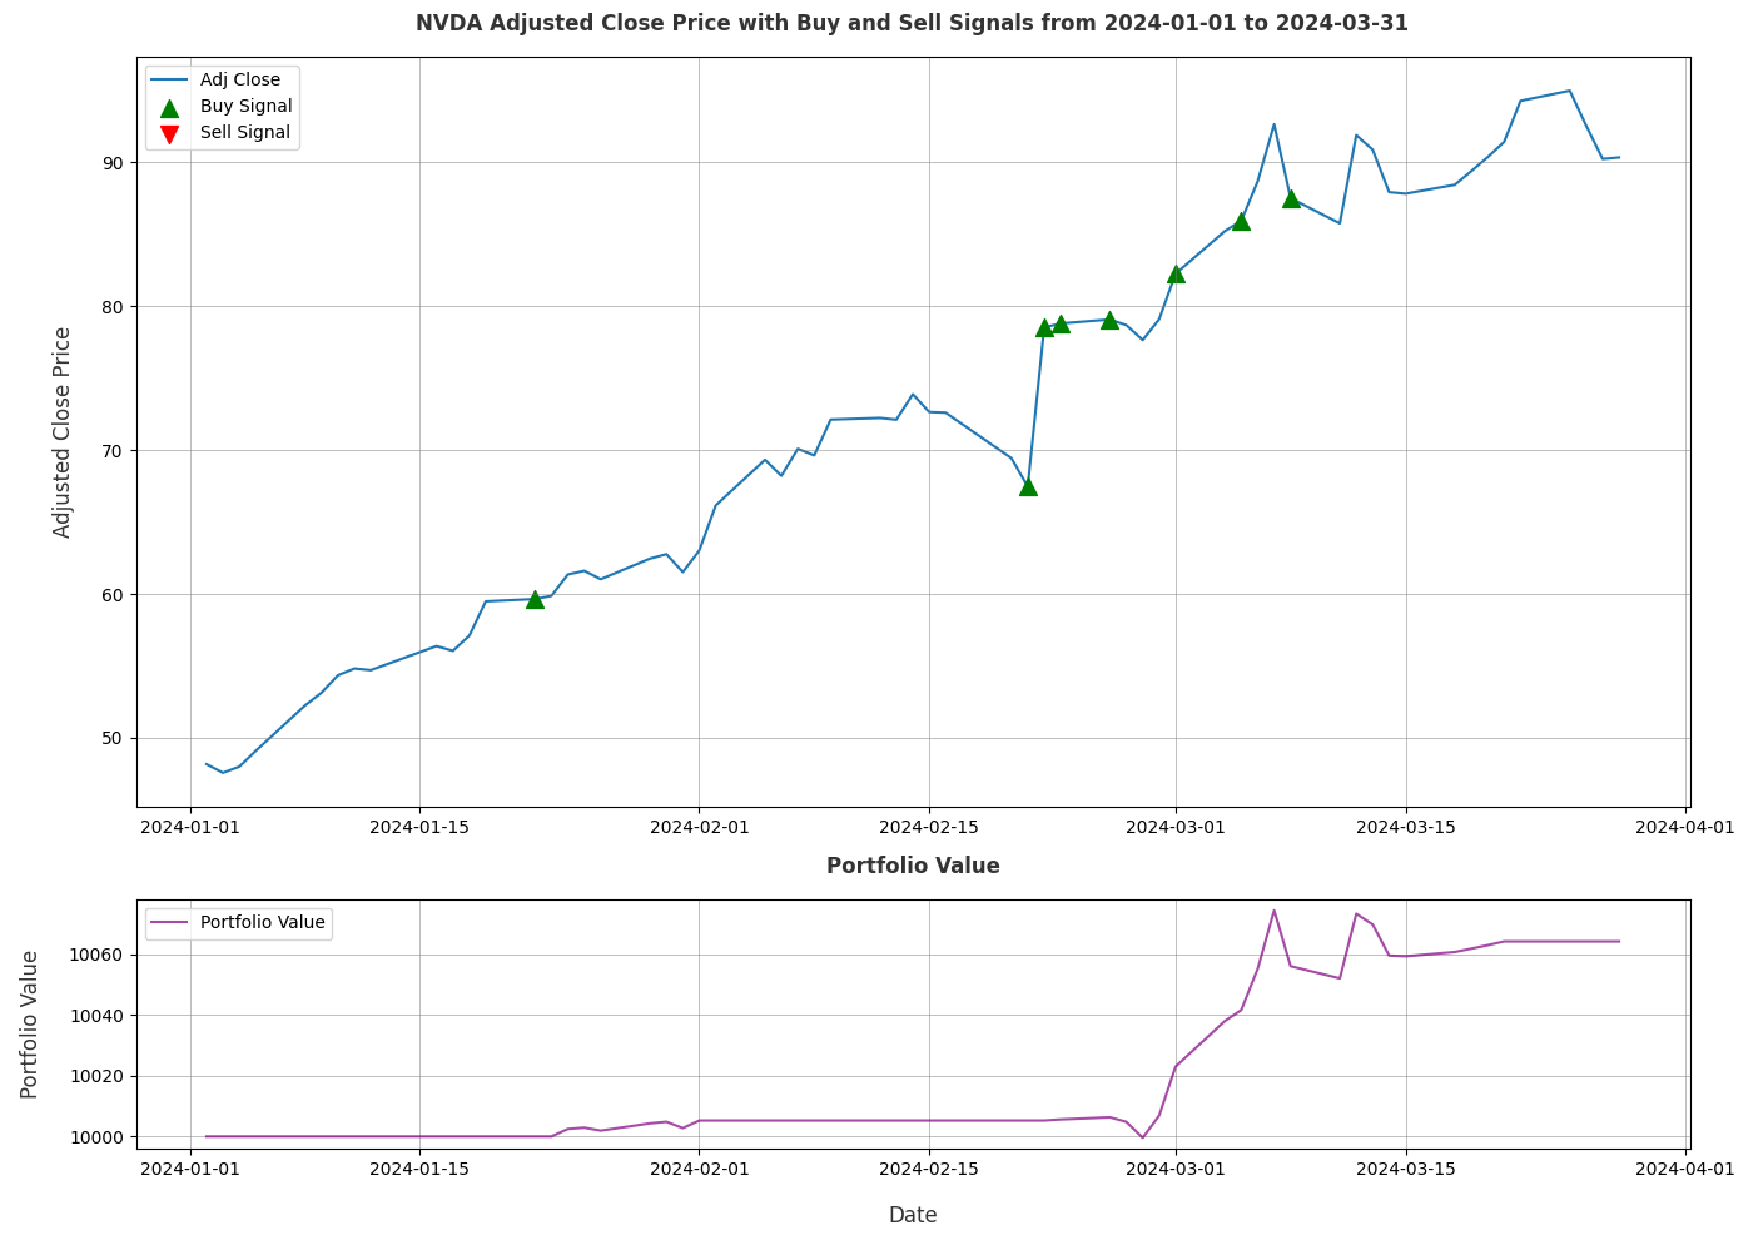
\includegraphics[width=\textwidth]{img/experiment-stock/nvda-hold-strategy-a.pdf}
    \caption{Nvidia Corp. (NVDA) adjusted close price with buy and sell signals in the first quarter of 2024. Hold strategy based on sentiment signals.}
    \label{fig:elsa-experiment-stock-nvda-hold-strategy}
\end{figure}

\begin{figure}[hbp]
    \centering
    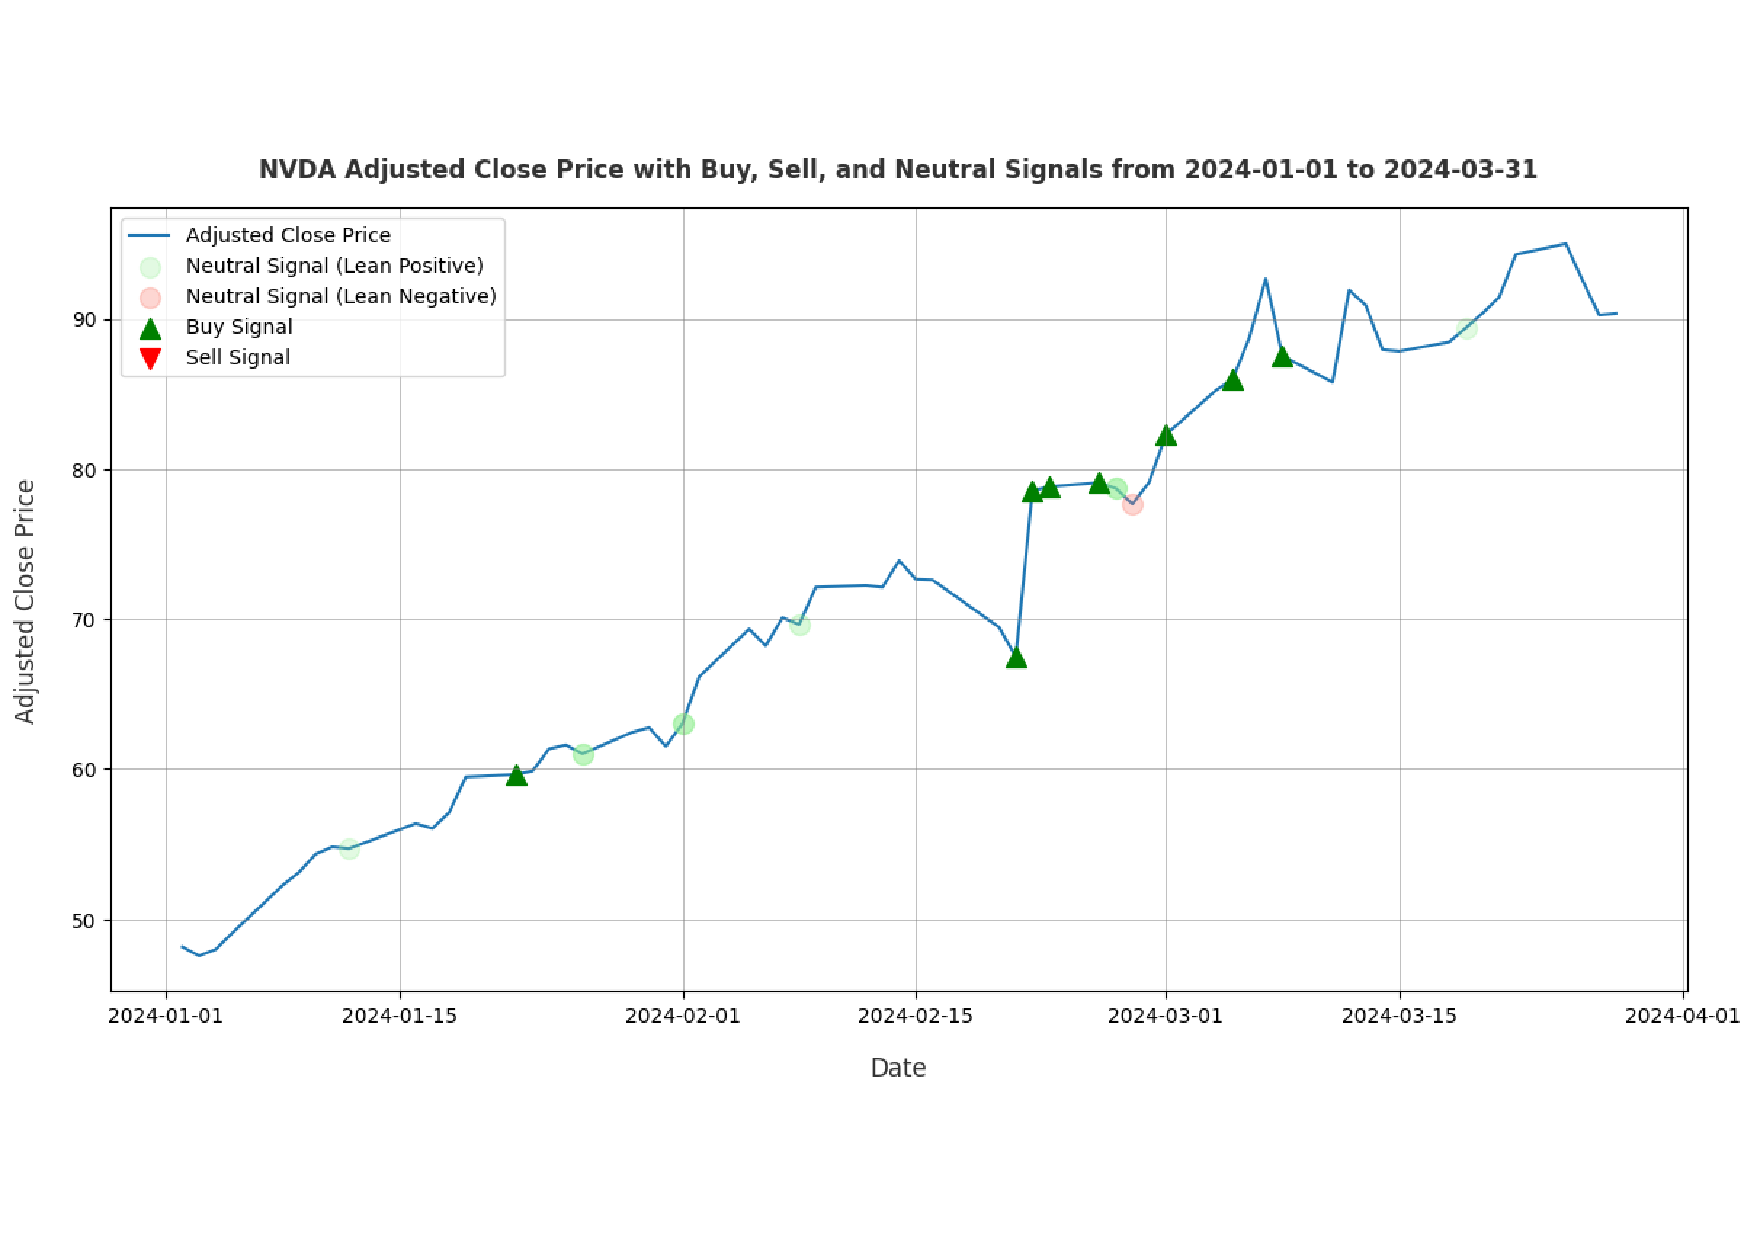
\includegraphics[width=\textwidth]{img/experiment-stock/nvda-neutral-a.pdf}
    \caption{Nvidia Corp. (NVDA) adjusted close price with the buy, sell and neutral signals in the first quarter of 2024.}
    \label{fig:elsa-experiment-stock-nvda-neutral}
\end{figure}

Our aim is not to create the perfect investment strategy but to provide a foundational understanding of using sentiment data. Focusing on the data related to Nvidia and its sentiment distribution after aggregation (Figure \ref{fig:elsa-experiment-stock-nvda-comparison}), we notice frequent occurrences of neutral sentiment values, which we exclude from our strategy. To maximise the utility of the data when encountering neutral classifications, we refine the approach. If the positive sentiment value exceeds the negative sentiment value, we classify it as neutral lean positive. Otherwise, it is classified as neutral lean negative. The Nvidia with neutral categories results are shown in Figure \ref{fig:elsa-experiment-stock-nvda-neutral}.

\begin{figure}[hb]
    \centering
    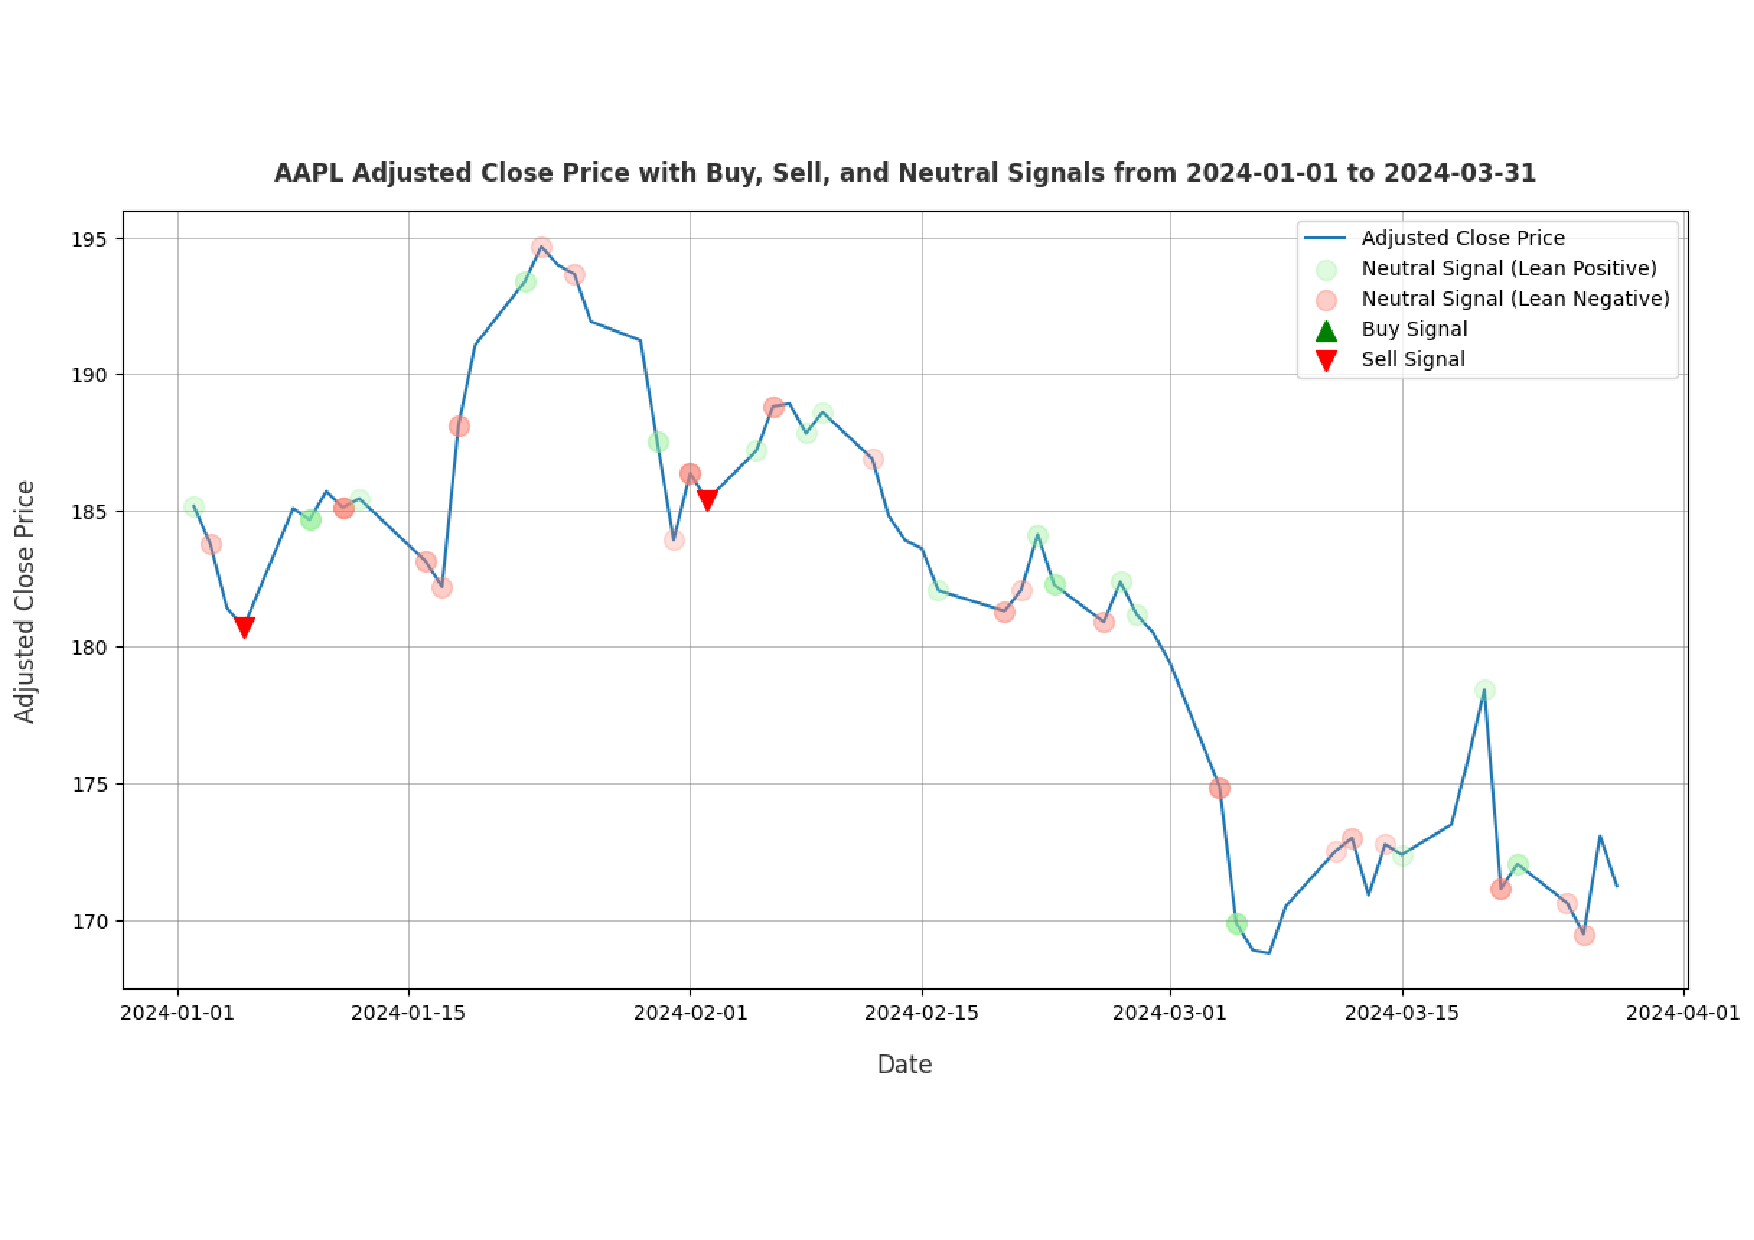
\includegraphics[width=\textwidth]{img/experiment-stock/aapl-neutral-a.pdf}
    \caption{Apple Inc. (AAPL) adjusted close price with the buy, sell and neutral signals in the first quarter of 2024.}
    \label{fig:elsa-experiment-stock-aapl-neutral}
\end{figure}

For a more precise illustration of neutral sentiment projection, we apply it to Apple Inc. (AAPL), as depicted in Figure \ref{fig:elsa-experiment-stock-aapl-neutral}. This technique ensures that even neutral sentiments are interpreted to maximise the data's potential. Additionally, the sentiment value adjusts the colour's alpha channel, increasing it by approximately $0.25$ for better visibility. This procedure allows us to intentionally overlook sentiments with high neutral values and low positive and negative values. We ensure that the most relevant sentiments are highlighted, enhancing the clarity and effectiveness of our analysis. Testing the strategy and displaying neutral sentiment for other companies, such as Apple, Amazon.com Inc. (AMZN), Alphabet Inc. (GOOGL), Meta Platforms Inc. (META), Microsoft Corp. (MSFT), and Tesla Inc. (TSLA), we obtain the results shown in Appendix \ref{appsec:hold-strategy}. The results demonstrate the effectiveness of our approach using buy and sell signals. There is potential for further development in employing neutral sentiment.

\subsection{Correlation}
\label{subsec:elsa-correlation}
Considering the correlation between sentiment and adjusted close price is appropriate to avoid concluding and provide an independent view based on the chosen market strategy. First, we will focus on the correlation between sentiment and the stock price of Nvidia. Recalling the sentiment distribution after aggregation in Figure \ref{fig:elsa-experiment-stock-nvda-aggregated}, which we extend to include neutral categories lean positive and lean negative, all sentiment data are interpolated using the previous day method, see Figure \ref{fig:elsa-experiment-stock-nvda-interpolated}. The strategy initially focused solely on positive and negative sentiments, but we are also interested in neutral sentiment for correlation purposes.

\begin{figure}[htbp]
    \centering
    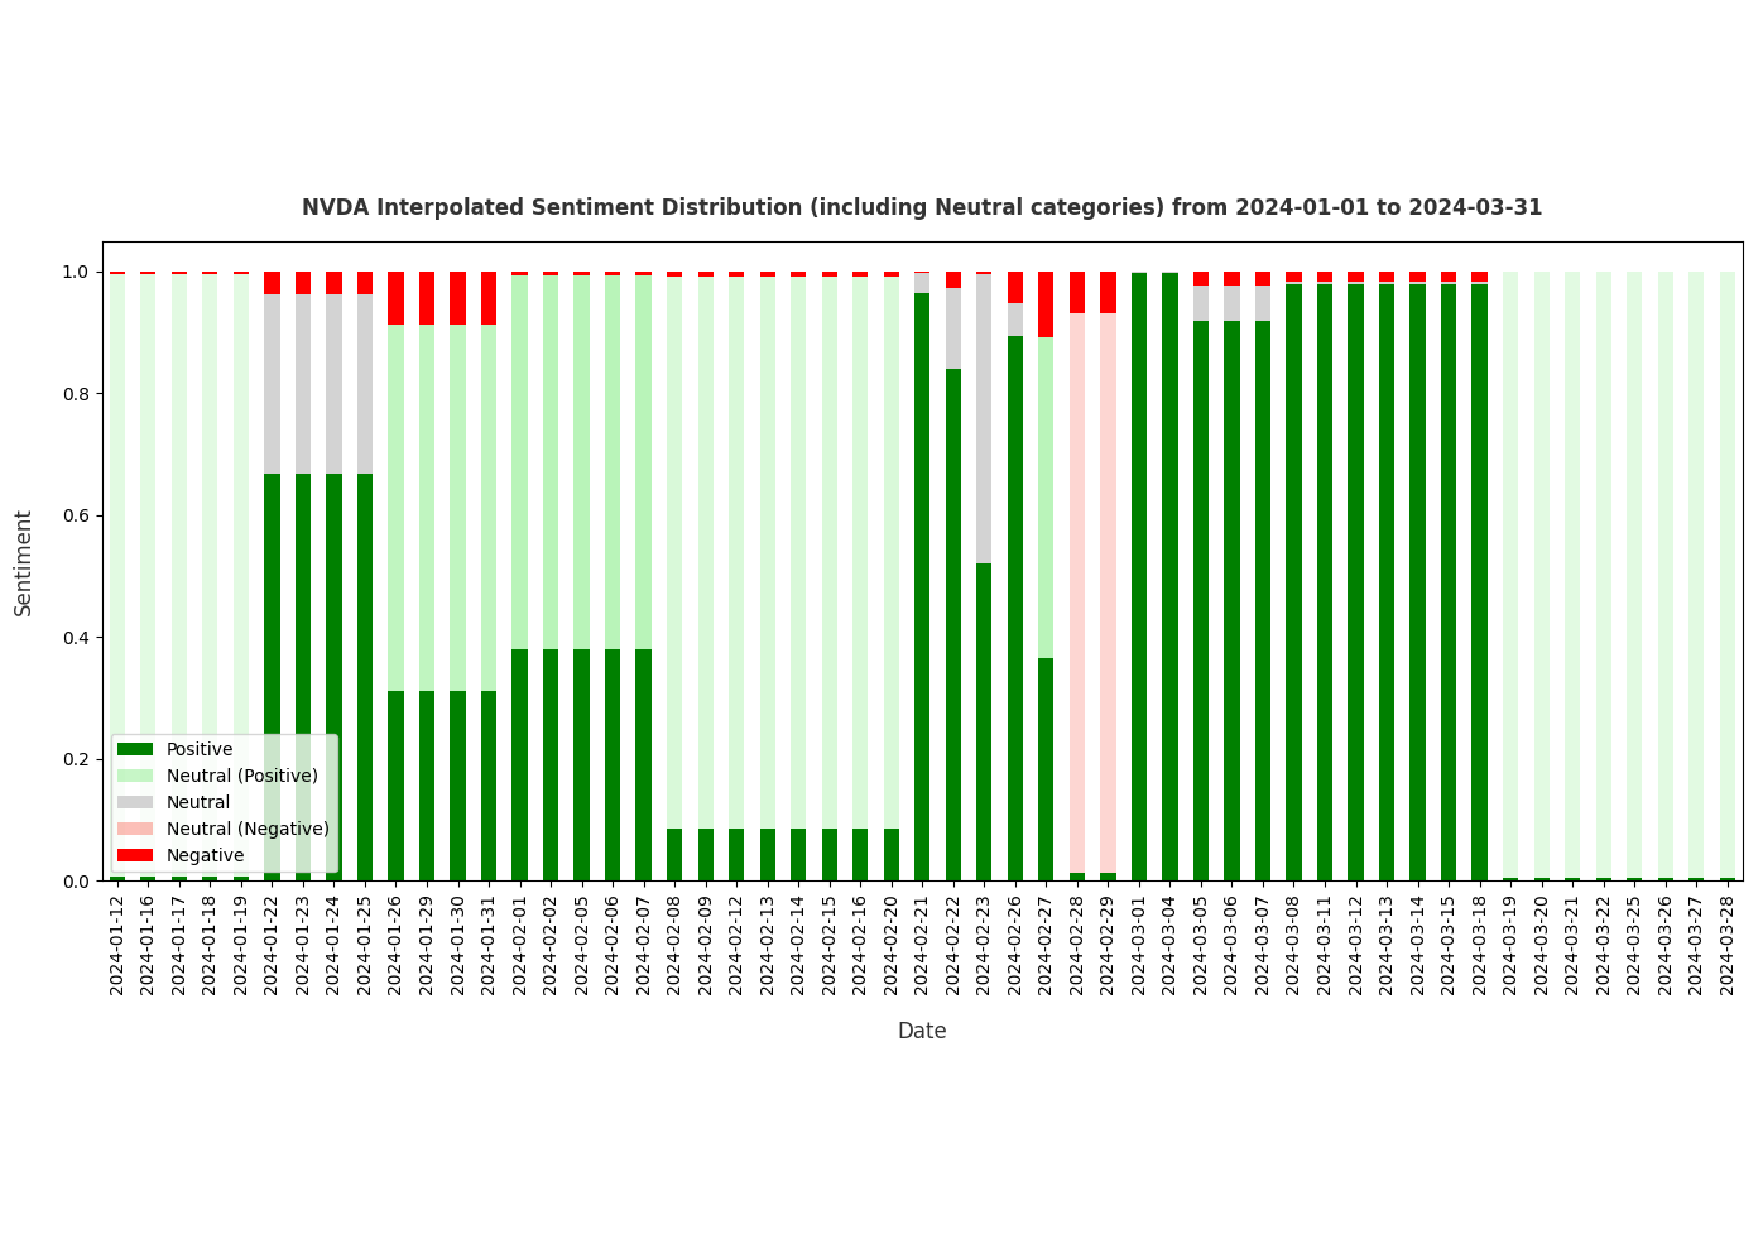
\includegraphics[width=\textwidth]{img/experiment-stock/nvda-interpolated-a.pdf}
    \caption{Nvidia Corp. (NVDA) adjusted close price with interpolated sentiment in the first quarter of 2024.}
    \label{fig:elsa-experiment-stock-nvda-interpolated}
\end{figure}

The choice of interpolation method is based on the policy that if sentiment data are missing for a given day, we use the values from the previous day. This approach is chosen because it aligns with sentiment behaviour. For instance, linear interpolation could be chosen if sentiment changes were expected to be linear, which is unrealistic. Using the previous day method allows us to simulate that the company sentiment remains the same if no new sentiment data are available. 

A negative correlation between negative sentiment and adjusted close price suggests that the adjusted close price tends to decrease as negative sentiment increases. Conversely, the adjusted closing price tends to increase as negative sentiment decreases. This negative correlation indicates an inverse relationship between these variables. Therefore, negative and neutral lean negative sentiments in the results are inverted. The correlation results between sentiments and Nvidia's adjusted close price are shown in Figure \ref{fig:elsa-experiment-stock-nvda-corr}. The results show a positive correlation with a value of about $0.25$ in three sentiment cases, which means a successful correlation between sentiment and stock prices. In the case of lean negative, the correlation is negative, which means that the adjusted close price increases as negative sentiment grows. The correlations of other companies are shown in Appendix \ref{appsec:correlation}.

\begin{figure}[ht]
    \centering
    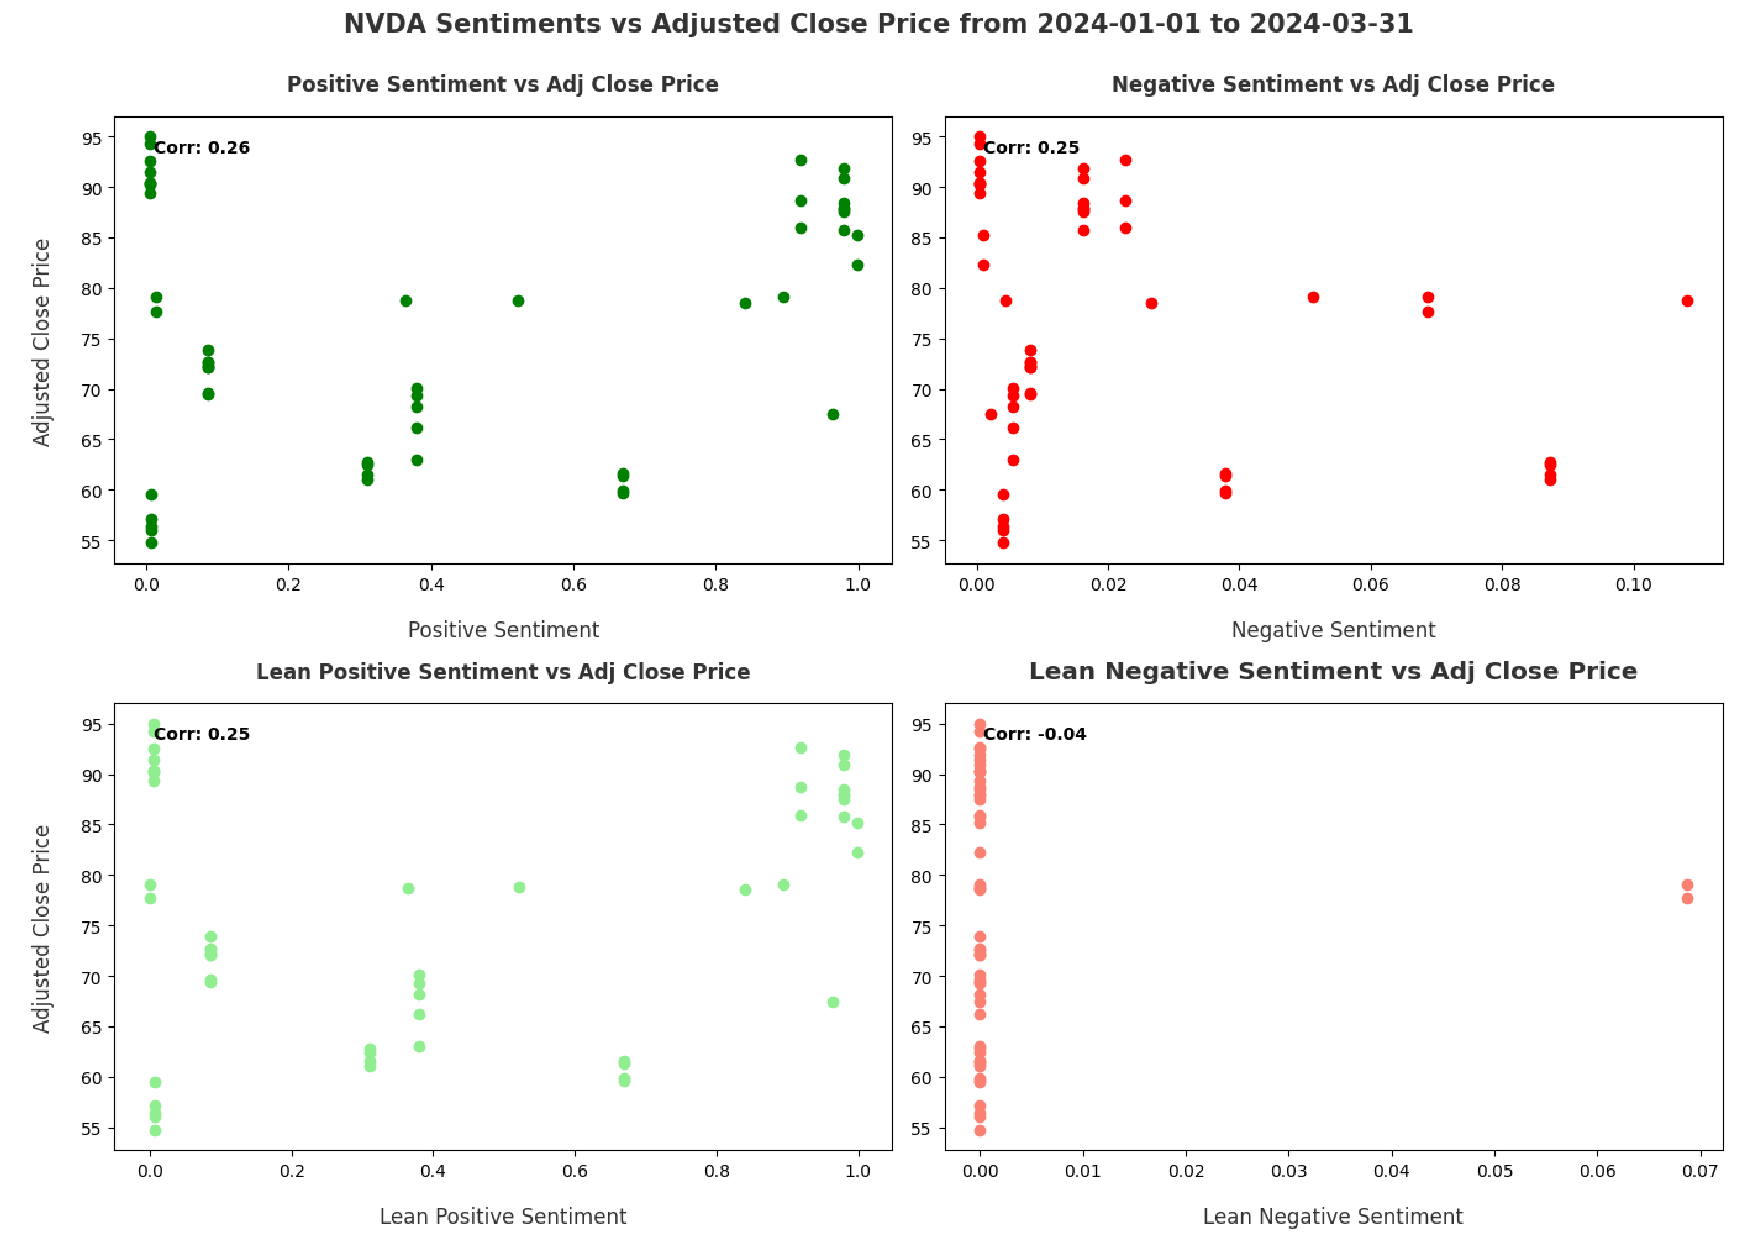
\includegraphics[width=\textwidth]{img/experiment-stock/nvda-corr-a.pdf}
    \caption{Nvidia Corp. (NVDA) sentiment correlation with adjusted close price in the first quarter of 2024.}
    \label{fig:elsa-experiment-stock-nvda-corr}
\end{figure}

If we look at both the strategy and the correlation analysis results, they are slightly satisfactory. The strategy employs a straightforward approach and does not account for other factors that could influence stock prices. High negative or positive sentiment is thus partly a reaction to stock prices and partly an influence of them. For better accuracy, setting a threshold for classifying a given sentiment could help raise the level of sentiment required to be considered purely positive or negative. Neutral sentiment also plays a role and can be helpful in certain situations, as confirmed by the correlation with the adjusted close price.

The sum of the profits from portfolios based on this strategy is positive. We achieved a total return of about $0.74\%$, which amounted to approximately $\$74$ profit. Although there were more loss-making positions than profitable ones, the losses were minor compared to the more significant profits. If we had more articles available in given time period, there would undoubtedly be more opportunities, but the question remains whether they would be reliable and not too numerous. We should set a boundary for when we are willing to enter positions.

Regarding the correlation analysis, the results confirm that utilising the full potential of negative and positive sentiment data in classifying neutral sentiment is sensible. Additionally, some correlation, albeit small, does exist and is mostly positive. This indicates that sentiment can be a good indicator of stock prices. It is important to remind readers not to be misled when comparing the strategy portfolio and correlation results, as the portfolio value is based on positive and negative sentiment, and positions are held for seven days. The results are thus rather satisfactory. However, further experiments with more data and different strategies, additional indicators, and conceivably a different interpolation method in the case of correlation would be appropriate.

